
\documentclass[conference]{IEEEtran}
\usepackage{stmaryrd}
\usepackage{amsfonts}
% If the IEEEtran.cls has not been installed into the LaTeX system files,
% manually specify the path to it: e.g.,
% \documentclass[conference]{../sty/IEEEtran}

\usepackage{graphicx,times,psfig,amsmath} % Add all your packages here

% correct bad hyphenation here
\hyphenation{op-tical net-works semi-conduc-tor IEEEtran}

\IEEEoverridecommandlockouts    % to create the author's affliation portion
                % using \thanks

\textwidth 178mm    % <------ These are the adjustments we made 10/18/2005
\textheight 239mm   % You may or may not need to adjust these numbers again
\oddsidemargin -7mm
\evensidemargin -7mm
\topmargin -6mm
\columnsep 5mm

\begin{document}


% paper title: Must keep \ \\ \LARGE\bf in it to leave enough margin.
\title{\ \\ \LARGE\bf A K-Winners-Take-All Neural Network Based on Linear Programming Formulation\thanks{Shenshen Gu and Jun Wang are with the Department of Mechanical and Automation Engineering, The Chinese University of Hong Kong, Shatin, New Territories, Hong Kong (email: \{ssgu, jwang\}@mae.cuhk.edu.hk).} \thanks{This work was supported by a CUHK Direct Grants under Project Code
2050375}}

\author{Shenshen Gu and Jun Wang}

% avoiding spaces at the end of the author lines is not a problem with
% conference papers because we don't use \thanks or \IEEEmembership
% use only for invited papers
%\specialpapernotice{(Invited Paper)}

% make the title area
\maketitle

\begin{abstract}
In this paper, the K-Winners-Take-All (KWTA) problem is formulated
equivalently to a linear program. A recurrent neural network for
KWTA is then proposed for solving the linear programming problem.
The KWTA network is globally convergent to the optimal solution of
the KWTA problem. Simulation results are further presented to show
the effectiveness and performance of the KWTA network.
\end{abstract}

% no key words

\section{Introduction}


\PARstart{W}{inner-take-all} (WTA) is an operation that identifies
the largest value from multiple input signals. Such an operation has
many applications in a variety of fields including associative
memories \cite{cit:1}, cooperative models of binocular stereo
\cite{cit:2}, Fukushima's neocognitron for feature extraction, and
ect \cite{cit:3}.

As an extension of winner-take-all operation, k-winners-take-all
(KWTA) selects the $k$ largest inputs from the total $n$ inputs. It
can be considered as a generalized form of winner-take-all
operation. It has recently been reported that KWTA is computational
powerful compared with the standard neural network models with
threshold logic gates \cite{cit:4}\cite{cit:5}. Any boolean function
can be computed by a single k-winners-take-all unit applied to
weighted sums of input variables. Beside the applications in neural
network model, KWTA operation has important applications in machine
learning, such as k-neighborhood classification, k-means clustering,
etc. As the number of inputs becomes large and/or the selection
process should be operated in real time, parallel algorithms and
hardware implementation are desirable. For these reasons, there have
been many attempts to design very large scale integrated (VLSI)
circuits to perform KWTA operations \cite{cit:6}--\cite{cit:29}.

Unlike the traditional KWTA networks that utilize the concept of
mutual inhibition, this paper presents a neural network
implementation of KWTA operation based on the linear optimization
formulation, which has the $O(N)$ complexity. For this neural
network, global convergence is guaranteed and time-varying signals
can be tackled.

The rest of this paper is organized as follows: Section II derives
an equivalent linear programming (LP) formulation of KWTA, which is
suitable for the neural network design. Section III introduces the
neural network design procedure, architecture and properties. Some
simulation results are presented in Section IV to show its
performance. Finally, Section V concludes the paper.


\section{Equivalent Reformulations}

Mathematically, KWTA operation can be formulated as a function as
follows:

\begin{equation}
x_i=\left\{ \begin{array}{ll} 1, & \textrm{if $v_i$$\in$\{$k$ largest elements of $v$\}; }\\
0, & \textrm{otherwise;}\end{array}\right. \label{eq:eq1}
\end{equation} for $i=1,\ldots,n$; where $v\in R^{n}$ and $k\in
\{1,\ldots,n-1 \}$.

\begin{figure}[htp]
\centerline{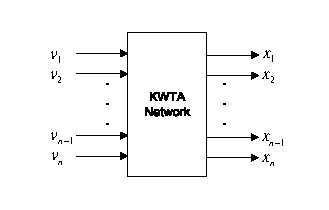
\includegraphics[width=2.6in]{KWTA.eps}} \caption{The
diagram of KWTA operation} \label{fig_sim}
\end{figure}

The function (\ref{eq:eq1}) can be further express by the following
integer program:

\begin{equation}
\begin{array}{lll}
&\mbox{minimize}&\quad -v^{T}x,\\
&\mbox{subject to}&\quad e^{T}x=k, \\
&\mbox{}&\quad x_i\in\{0,1\},\   i=1,2,\ldots ,n;
\end{array}
\label{eq:eq2}
\end{equation}
where $v=[v_1,\ldots,v_n]^{T},\ e=[1,\ldots,1]^{T}\in R^{n},\
x=[x_1,\ldots,x_n]^{T}\in R^{n}$ and $k$ is a nonnegative integer
less than $n$.

Fig. 1 shows the KWTA operation graphically. In this section, we
will formulate the KWTA operation as a linear programming problem,
which is suitable for neural network design. Toward this objective,
we should prove the following theorem.

\textit{Theorem 1:} The solution of (\ref{eq:eq2}) is equivalent to
the solution $x^{*}$ of the following linear programming problem (3)
.

\begin{equation}
\begin{array}{lll}
&\mbox{minimize}&\quad -v^{T}x,\\
&\mbox{subject to}&\quad e^{T}x=k, \\
&\mbox{}&\quad x_i\in[0,1],\   i=1,2,\ldots ,n.
\end{array}
\label{eq:eq11}
\end{equation}

\textit{Proof:} Since $e$ is an $n$-dimensional column vector with
all its elements are $1$s. Therefore, in this special case, every
square submatrix of $e$ has determinant equals to $1$. As such,
vector $e$ is said to be totally unimodular. In addition, $k$ is an
integer. As a result of the totally unimodular property, we can get
the conclusion that the optimum solution to problem (3) is
equivalent to the solution of problem (2). The proof is complete.

From the above proof, it can be easily found that we can design a
KWTA neural network by solving the LP problem (3). As a basic
optimization problem, there are a lot of algorithms for solving the
LP problem. But traditional algorithms typically involve an
iterative process, and long computational time limits their usage.
For this reason, the optimization capability of the recurrent neural
network has been widely investigated and have shown promise for
solving optimization problems more effectively. After the seminal
work of Tank and Hopfield \cite{cit:14}\cite{cit:15}, various neural
network models for optimization have been proposed. They can be
categorized as the penalty-parameter neural network \cite{cit:16},
the Lagrange neural network \cite{cit:17}, the deterministic
annealing neural network \cite{cit:18}, the primal-dual neural
network \cite{cit:19}\cite{cit:20} and the dual neural network
\cite{cit:30}\cite{cit:21}\cite{cit:22}.

\section{Model Description}

In recent decades, several effective recurrent neural networks for
solving linear programming problems have been proposed. In
\cite{cit:24}, a recurrent neural network for solving LP problems
with bounded variables is presented. For KWTA operation, the network
architecture has $n+1$ neurons (the number of integrators) and
$2n+1$ connections (the number of summers) and its dynamic equations
are as follows:

\begin{equation}
\left\{\begin{array}{l} \frac{dx}{dt}=\lambda \{ e(e^{T}x-k)-\|f(x+ey-v)-x\|_{2}^{2}(ey-v)\} \\
\frac{dy}{dt}=-\lambda\|f(x+ey-v)-x\|_{2}^{2}[ef(x+ey-v)-k]
\end{array} \right.
\label{eq:KWTA1}
\end{equation}
where $\lambda >0$ is a scaling constant, $x\in R^{n}$, $y\in R$,
$\|\cdot\|_{2}^{2}$ is the Euclidean norm and $f :R^{n}\to
[0,1]^{n}$ is a piecewise linear activation function which is
defined by $f (x)=[f(x_1),\ldots,f(x_n)]^{T}$ and

\begin{equation}
f(x_i)= \left\{ \begin{array}{ll} 0, & x_i <0;\\
x_i, & 0\le x_i\le 1;\\
1, & x_i >1.
\end{array}\right.
\end{equation}

The main drawback of this model is that the model should calculate
a higher-order term which degrades its speed and sensitivity.

In \cite{cit:25}, another recurrent neural network for LP problems
is presented. The architecture of this model for KWTA has $2n+1$
neurons and $3n+1$ connection and its dynamic equations are given as
following:

\begin{equation}
\left\{\begin{array}{l} \frac{dx}{dt}=-\lambda\{(v^{T}x+kz)v+e(e^{T}x-k)-(-2x)^{+}\}, \\
\frac{dy}{dt}=-\lambda \{(y-x)^{+}-e\}, \\
\frac{dz}{dt}=-\lambda\{(v^{T}x+kz)k-2e^{T}(ez-v)^{+}\},
\end{array} \right.
\label{eq:KWTA2}
\end{equation}
where $\lambda >0,$ $x\in R^{n}$, $y\in R^{n}$, $z\in R$,
$(x)^{+}=[(x_1)^{+},\ldots,(x_n)^{+}]^{T}$, and
$(x_i)^{+}=\max\{0,x_i\}$, $(i=1,\ldots,n)$.

In \cite{cit:26}, a recurrent neural network for solving nonlinear
convex programs subject to linear constraints is introduced. This
model can be converted to solve the LP problems. For KWTA operation,
since more $n$ variable should be use to act as slack variables, the
network architecture of this model has $2n+1$ neurons and $3n+1$
connections with the following dynamic equations:

\begin{equation}
\left\{\begin{array}{l} \frac{dx}{dt}=\lambda \{-x+(x+ez+v)^{+}\}, \\
\frac{dy}{dt}=\lambda \{(y-x)^{+}-e\}, \\
\frac{dz}{dt}=\lambda\{(e^{T}x-z)^{+}-k\},
\end{array} \right.
\label{eq:KWTA3}
\end{equation}
where $\lambda >0,$ $x\in R^{n}$, $y\in R^{n}$, and $z\in R$.

However, the above two models employ more neurons and connections to
accomplish the KWTA operation compared with the first model.

In \cite{cit:27}, a projection neural network to constrained
optimization problems is invented. This model can be used for
solving KWTA based on LP formulation with $n+1$ neurons and $2n+2$
connections. The procedure of constructing a neural network model
for solving problem (\ref{eq:eq11}) is given as follows:

Define a Lagrange function of (\ref{eq:eq11}) below

\begin{equation}
L(x,y)=-v^{T}x-y(e^{T}x-k)
\end{equation}
where $y\in R$ is referred to as the Lagrange Multiplier. According
to the Karush-Kuhn-Tucker (KKT) condition, $x^{*}$ is a solution to
(\ref{eq:eq11}) if and only if there exits $y^{*}\in R$ such that
$(x^{*},y^{*})$ satisfies the following condition:

\begin{equation}
\left\{\begin{array}{c} -v-ey\ge 0,\
x(-v-ey)=0,\\
e^{T}x-k=0,\ 0\le x\le 1.
\end{array} \right.
\end{equation}

Using the well-known projection theorem, we can easily obtain the
following Lemma.

\textit{Lemma 1:} $x^{*}$ is a solution to (\ref{eq:eq11}) if and
only if there exists $y^{*}\in R^{m}$ such that $(x^{*},y^{*})$
satisfies

\begin{equation}
\left\{\begin{array}{c} f (x+\alpha ey+\alpha v)-x=0,\\
e^{T}x-k=0,
\end{array} \right.
\end{equation}
where $\alpha$ is any positive constant.

\textit{Proof:} See \cite[pp. 267, Prop. 5.1]{cit:28}.

Based on the equivalent formulation in Lemma 1, we propose a
recurrent neural network for KWTA operation with its dynamical
equations as follows:

\begin{equation}
\left\{\begin{array}{l} \frac{dx}{dt}=\lambda \left( -x+f (x+\alpha ey+\alpha v)\right),\\
\frac{dy}{dt}=\lambda (e^{T}x-k),
\end{array} \right.
\label{eq:KWTA4}
\end{equation}
where $\lambda >0$, $\alpha >0$, $x\in R^{n}$, $y\in R$.

The element-form of the dynamic equation (\ref{eq:KWTA4}) can be
described as follows:

\begin{equation}
\left\{\begin{array}{l} \frac{dx_i}{dt}=\lambda \left( -x_i+f (x_i+\alpha y+\alpha v_i)\right),\ i=1,\ldots,n;\\
\frac{dy}{dt}=\lambda (\sum_{i=1}^{n}x_i-k).
\end{array} \right.
\end{equation}


In \cite{cit:27}, it is proved that this network is globally
exponentially stable. The dynamics can be easily realized in a
recurrent neural network with a single-layer structure as shown in
Fig. 2, where $\lambda =1$, $\alpha =1$ and $f(\cdot)$ can be
implemented by using a piecewise linear activation function. As
shown in Fig. 2, a circuit implementing this network consists of
$2n+1$ summers, $n+1$ integrators and $n+1$ operational amplifiers.

\begin{figure}[htp]
\centerline{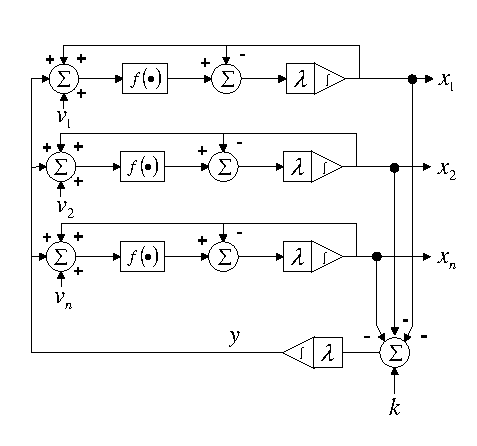
\includegraphics[width=3.0in]{Archi.eps}}
\caption{Architecture of the KWTA network} \label{fig 2}
\end{figure}

The number of neurons and connections of these models are listed in
Table I. From this table, it is clear that the model proposed in
\cite{cit:27} has a low model complexity. For this reason, we adopt
this model for KWTA operation.

\begin{table}[h]
\caption{Model complexity of four recurrent neural networks for KWTA
operation based on Linear programming formulation}
\begin{center}
\begin{tabular}{|c|c|c|c|}
\hline
\multicolumn{1}{|c|}{Model}% time}
& \multicolumn{1}{|c|}{Eqn}% time}
& \multicolumn{1}{|c|}{Neurons}% time}
& \multicolumn{1}{|c|}{Connections} \\% cost}\\
%\hline
 \hline
 \cite{cit:24} & (\ref{eq:KWTA1}) &  $n+1$  &  $2n+1$\\ \hline
 \cite{cit:25} & (\ref{eq:KWTA2}) &  $2n+1$  &  $3n+1$\\ \hline
 \cite{cit:26} & (\ref{eq:KWTA3}) &  $2n+1$  &  $3n+1$\\ \hline
 \cite{cit:27} & (\ref{eq:KWTA4}) &  $n+1$  &  $2n+1$  \\ \hline
\end{tabular}
\label{tab-liu2}
\end{center}
\end{table}

\section{Simulation Results}

To show the effectiveness and efficiency of the proposed KWTA neural
network, the following four simulations are performed.

In the first simulation, the inputs are set to be $v_i=i$,
$(i=1,2,3,4)$ and $k=2$; that is, select two largest signals from
the inputs. The transient behaviors of $x$ are shown in Fig. 3. It
can be seen that the steady outputs are $[0\ 0\ 1\ 1]^{T}$. This
means two largest elements; i.e., $v_3$ and $v_4$ are successfully
selected. From the figure, it is also obvious that the neural
network can quickly converge to the desired equilibria once the
inputs are imposed.

\begin{figure}[htp]
\centerline{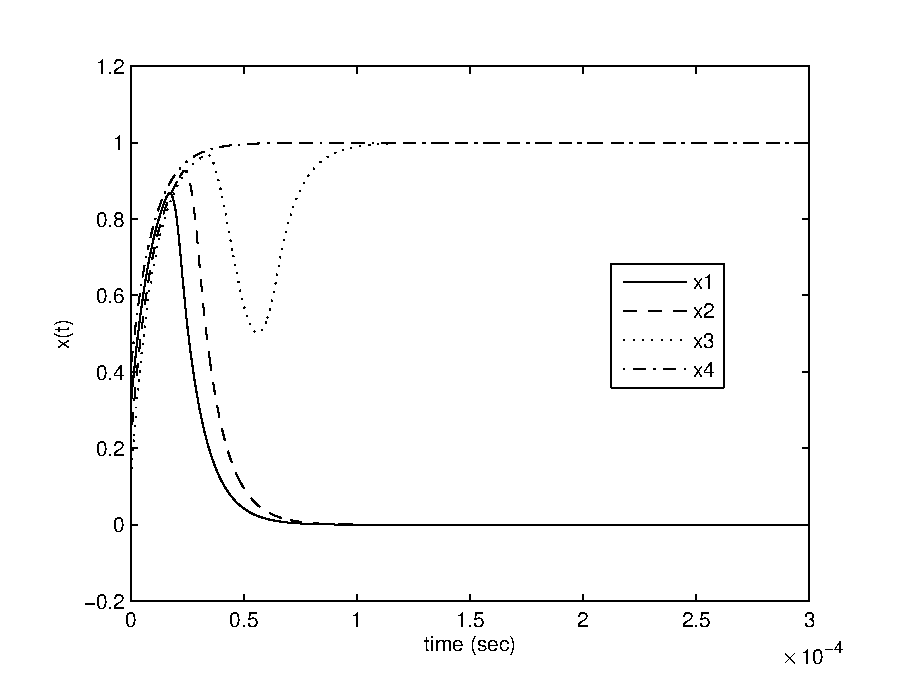
\includegraphics[width=3.9in]{dynamic.eps}}
\caption{Transient behavior of $x$} \label{fig_3}
\end{figure}

In the second simulation, consider 4 sinusoidal input signals
ranged from $-1$ to $1$ with constant phase difference and $k=2$.
Fig. 4 illustrates the 4 input signals and the transient outputs
of the KWTA network. The simulation results show that the KWTA
network can effectively determine the two largest signals from the
time-varying signals in real time.

\begin{figure}[htp]
\centerline{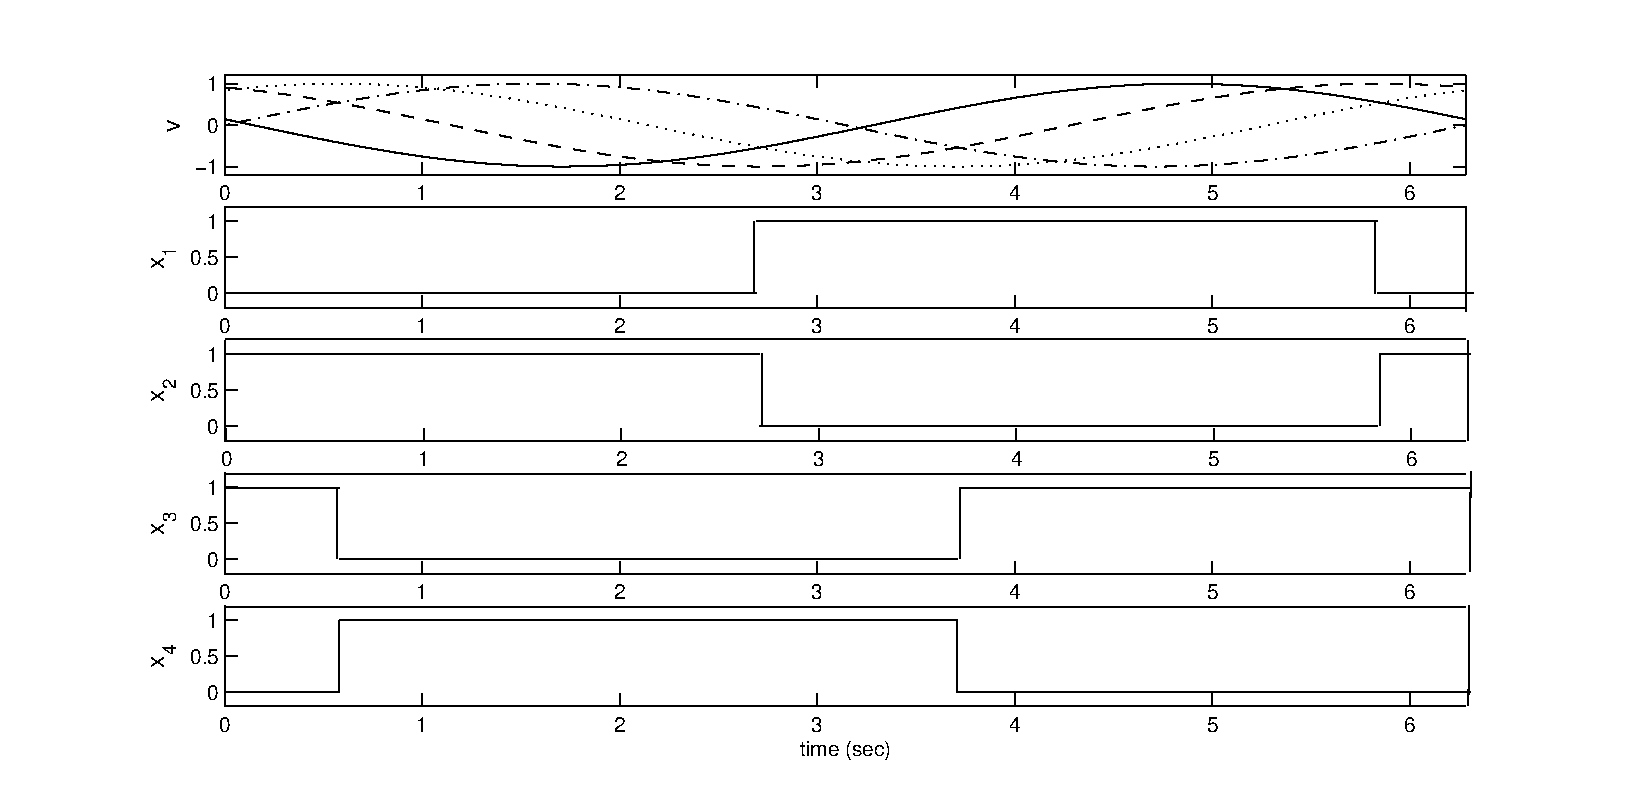
\includegraphics[width=3.7in]{sinu.eps}}
\caption{Sinusoids inputs and generated outputs of the KWTA network}
\label{fig_4}
\end{figure}

\begin{figure}[htp]
\centerline{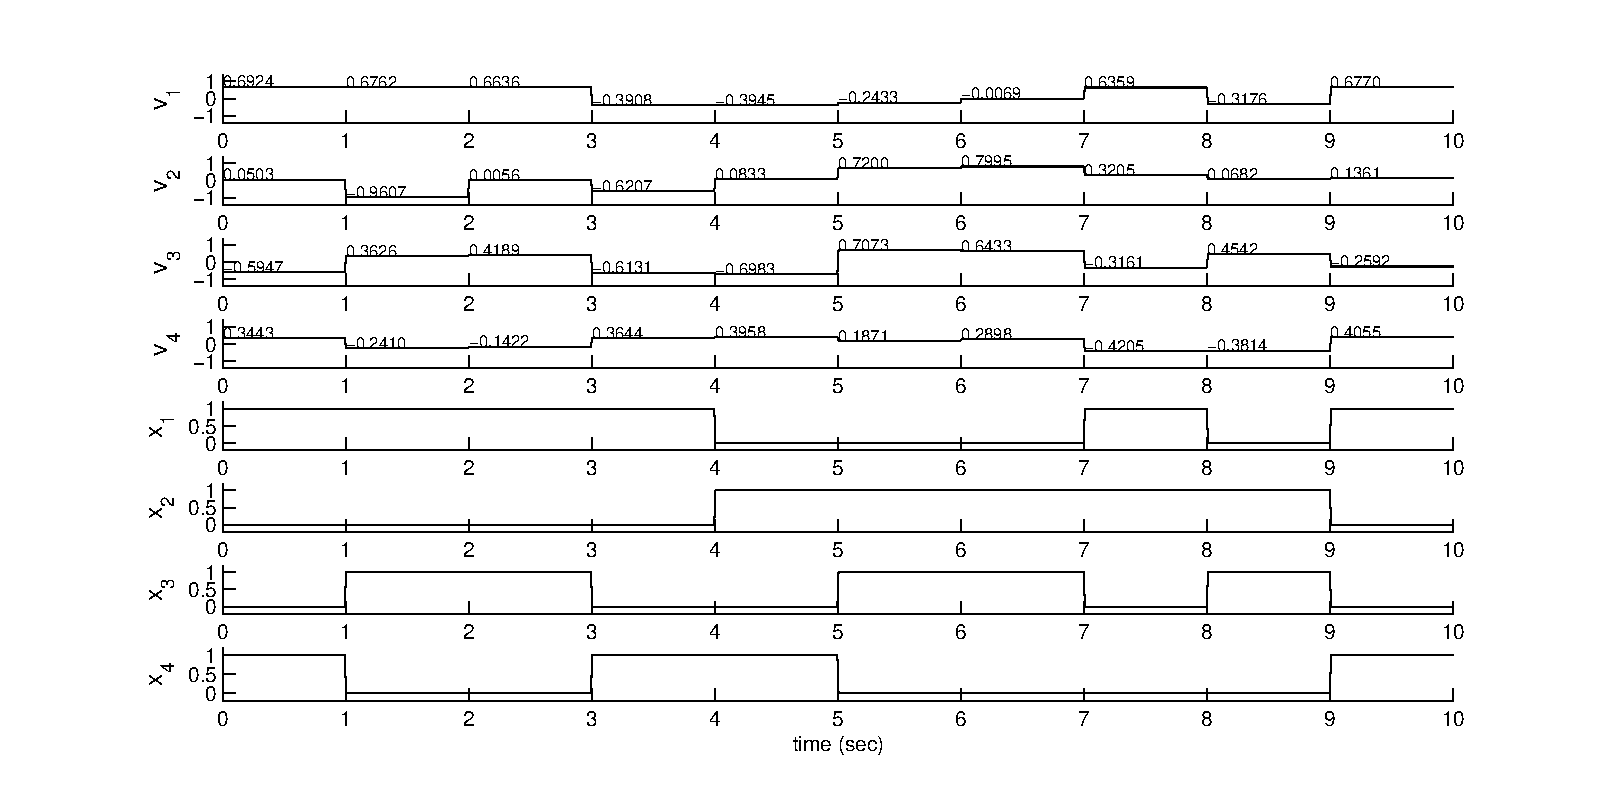
\includegraphics[width=3.7in]{ramdon10.eps}}
\caption{Random inputs and generated outputs of the KWTA network}
\label{fig_5}
\end{figure}

In order to test the response of the model to random input signals,
we further show the following experimental results. In this test,
four random signals ranged under uniform distribution from $-1$ to
$1$ are generated and fed into the KWTA neural network. The neural
network is regulated to determine the two largest signals at any
time. Fig. 5 shows that the KWTA network can output the correct
results in the whole period. It means that this model has good
response property to random inputs.



Finally, in order to reveal that the KWTA network has good
performance to solve the high-dimensional problems, Fig. 6 shows the
simulation results of the KWTA network with 5, 10, 15 and 20 inputs
where $\alpha=1,\ \lambda=10^{5}$. It is demonstrated that the
convergence rate of the KWTA network is independent of $n$.


\begin{figure}[htp]
\centerline{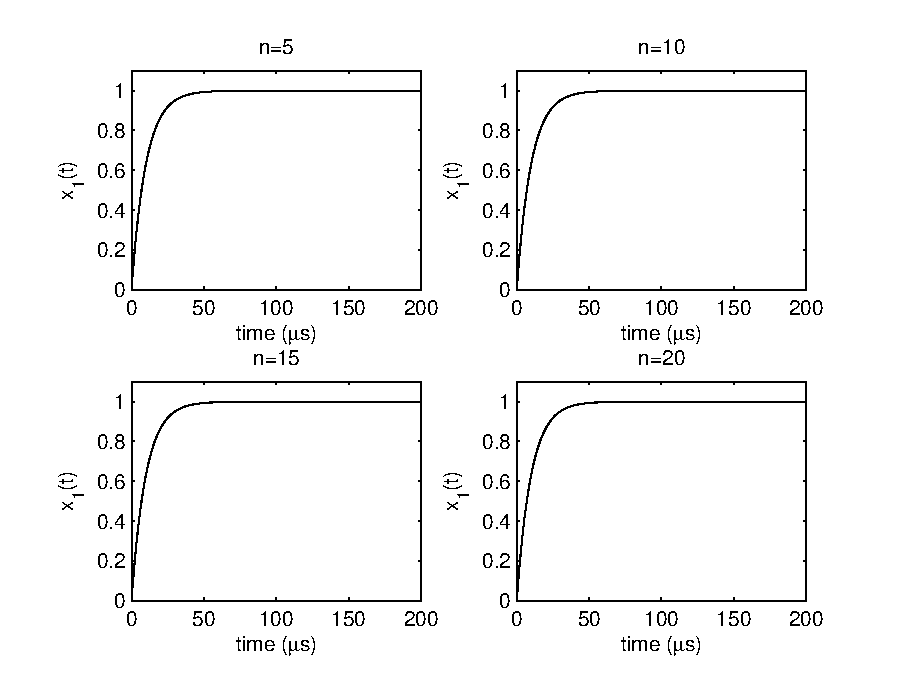
\includegraphics[width=3.6in]{micro.eps}}
\caption{Responses of the KWTA network to different number of
inputs} \label{fig_5}
\end{figure}

\section{Conclusions}
A KWTA network is developed for K-winners-take-all operation based
on a linear programming formulation. The KWTA network is shown to be
stable and can perform the KWTA operation in real time. The KWTA
network is also demonstrated to be capable of solving
high-dimensional KWTA problems. In addition, compared with several
existing neural networks, the KWTA network proposed has the simplest
architecture.


% trigger a \newpage just before the given reference
% number - used to balance the columns on the last page
% adjust value as needed - may need to be readjusted if
% the document is modified later
%\IEEEtriggeratref{8}
% The "triggered" command can be changed if desired:
%\IEEEtriggercmd{\enlargethispage{-5in}}

% references section
% NOTE: BibTeX documentation can be easily obtained at:
% http://www.ctan.org/tex-archive/biblio/bibtex/contrib/doc/

% can use a bibliography generated by BibTeX as a .bbl file
% standard IEEE bibliography style from:
% http://www.ctan.org/tex-archive/macros/latex/contrib/supported/IEEEtran/testflow/bibtex
%\bibliographystyle{IEEEtran.bst}
% argument is your BibTeX string definitions and bibliography database(s)
%\bibliography{IEEEabrv,../bib/paper}
%
% <OR> manually copy in the resultant .bbl file
% set second argument of \begin to the number of references
% (used to reserve space for the reference number labels box)


\def\V{\rm vol.~}
\def\N{no.~}
\def\pp{pp.~}
\def\Pot{\it Proc. }
\def\IJCNN{\it International Joint Conference on Neural Networks\rm }
\def\ACC{\it American Control Conference\rm }
\def\SMC{\it IEEE Trans. Systems\rm , \it Man\rm , and \it Cybernetics\rm }

\def\handb{ \it Handbook of Intelligent Control: Neural\rm , \it
    Fuzzy\rm , \it and Adaptive Approaches \rm }

\begin{thebibliography}{22}
\bibitem{cit:1} A. Krogh, J. Hertz and R.G. Palmer,
        {\it Introduction to the Theory of Neural Computation.}
        Addison-Wesley, Redwook City, CA, 1991.

\bibitem{cit:2} D. Marr and T. Poggio, ``Cooperative computation of stereo disparity,"
        {\it Science}, vol. 195, pp. 283-328, 1977.

\bibitem{cit:3} A.L. Yuille and D. Geiger,
        {\it The Handbook of Brain Theory and Neural Networks.}
        Chapter Winner-Take-All Networks, pp. 1228-1231, The MIT Press, 2 edition, 2002.

\bibitem{cit:4} W. Maass, ``Neural computation with winner-take-all as the only nonlinear
operation,"
        {\it Advances in Neural Information Processing Systems}, vol. 12, 2000.

\bibitem{cit:5} W. Maass, ``On the computational power of
winner-take-all,"
        {\it Neural Computation}, vol. 12, pp. 2519-2535, 2000.

\bibitem{cit:6} W.J. Wolfe, D. Mathis, C. Anderson, J. Rothman, M. Gottler, G. Brady, R. Walker, G. Duane and G. Alaghband, ``K-winner networks,"
        {\it IEEE Transactions on Neural Networks}, vol. 2, pp. 310-315, Mar. 1991.

\bibitem{cit:7} J. Wang, ``Analogue winner-take-all neural networks for determining maximum and minimum signals,"
        {\it Int. J. Electronics}, vol. 77, no. 3, pp. 355-367, 1994.

\bibitem{cit:8} K. Urahama and T. Nagao, ``K-winners-take-all ciucuit with O(N) complexity,"
        {\it IEEE Transactions on Neural Networks}, vol. 6, pp. 776-778, May. 1995.

\bibitem{cit:9} B. Sekerkiran and U. Cilingiroglu, ``A CMOS k-winners-take-all circuit with O(N) complexity,"
        {\it IEEE Transactions on Circuits and Systems}, vol. 46, no. 1, Jan. 1999.

\bibitem{cit:10} Jayadeva and S.A. Rahman, ``A neural network with O(N) neurons for ranking N numbers in O(1/N) times,"
        {\it IEEE Transactions on Circuits and Systems I}, vol. 51, no. 10, Oct. 2004.

\bibitem{cit:11} J. Yen, J. Guo and H. Chen, ``A new k-winners-take-all neural network and its array architecture,"
        {\it IEEE Transactions on Neural networks}, vol. 9, no. 5. pp. 901-912, Sept. 1998.

\bibitem{cit:12} B.D. Calvert and C.A. Marinov, ``Another k-winners-take-all analog neural network,"
        {\it IEEE Transactions on Neural Networks}, vol. 11, no. 4, pp. 829-838, Jul. 2000.

\bibitem{cit:13} C.A. Marinov and B.D. Calvert, ``Performance analysis for a k-winners-take-all analog neural network: basic theory,"
        {\it IEEE Transactions on Neural Networks}, vol. 14, no. 4, pp. 766-780, Jul. 2003.

\bibitem{cit:29} C.A. Marinov and J.J. Hopfield, ``Stable computational dynamics for a class of circuits with O(N) interconnections capable of KWTA and rand extractions,"
        {\it IEEE Transactions on Circuits and Systems}, vol. 52, no. 5, pp. 949-959, May 2005.

\bibitem{cit:14} D.W. Tank and J.J. Hopfield, ``Simple neural optimization networks: An A/D converter, signal decision circuit, and a linear programming circuit,"
        {\it IEEE Transactions on Circuits and Systems}, vol. 33, no. 5, pp. 533-541, 1986.

\bibitem{cit:15} J.J. Hopfield and D.W. Tank, ``Computing with neural circuits: A model,"
        {\it Science}, vol. 233, pp. 625-633, 1986.



\bibitem{cit:30} S.B. Liu and J. Wang, ``A simplified dual neural network for quadratic programming with its KWTA application,"
        {\it IEEE Transactions on Neural Networks}, vol. 17, no. 6, pp. 1500-1510, Nov 2006.



\bibitem{cit:16} M.P. Kennedy and L.O. Chua, ``Neural networks for nonlinear programming,"
        {\it IEEE Transactions on Circuits and Systems}, vol. 35, no. 5, pp. 554-562, May. 1988.

\bibitem{cit:17} S. Zhang and A.G. Constantinides, ``Lagrange programming neural networks,"
        {\it IEEE Transactions on Circuits and Systems II}, vol. 39, no. 7, pp. 441-452, Jul. 1992.

\bibitem{cit:18} J. Wang, ``A deterministic annealing neural network for convex programming,"
        {\it Neural Networks}, vol. 5, no. 4, pp. 962-971, 1994.

\bibitem{cit:19} Y. Xia, ``A new neural network for solving linear and quadratic programming problems,"
        {\it IEEE Transactions on Neural Networks}, vol. 7, no. 6, pp. 1544-1547, Nov. 1996.

\bibitem{cit:20} Y. Xia, G. Feng and J. Wang, ``A primal-dual neural network for online resolving constrained kinematic redundancy in robot motion control,"
        {\it IEEE Transactions on Systems, Man and Cybernetics}, vol. 35, no. 1, pp.54-64, Feb. 2005.

\bibitem{cit:21} Y. Xia and J. Wang, ``A dual neural network for kinematic control of redundant robot manipulators,"
        {\it IEEE Transactions on Systems, Man and Cybernetics}, vol. 31, no. 1, pp.147-154, Feb. 2001.

\bibitem{cit:22} Y. Zhang and J. Wang, ``A dual neural network for convex quadratic programming subject to linear equality and inequality constraints,"
        {\it Physics Letters A}, pp. 271-278, Jun. 2002.

\bibitem{cit:23} S. Boyd and L. Vandenbeghe,
        {\it Convex Optimization.}
        Cambridge University Press, Cambridge, UK. 2004.

\bibitem{cit:24} Y. Xia and J. Wang, ``Neural network for solving linear programming problems with bounded variables,"
        {\it IEEE Transactions on Neural Networks}, vol. 6, no. 2, pp. 515-519, 1995.

\bibitem{cit:25} Y. Xia, ``A new neural network for solving linear programming problems and its application,"
        {\it IEEE Transactions on Neural Networks}, vol. 7, no. 2, pp. 525-529, 1996.

\bibitem{cit:26} Y. Xia and J. Wang, ``A recurrent neural network for solving nonlinear convex programs subject to linear constraints,"
        {\it IEEE Transactions on Neural Networks}, vol. 16, no. 2, pp. 378-386, 2005.

\bibitem{cit:27} Y. Xia and J. Wang, ``A general projection neural network for solving monotone variational inequalities and related optimization problems,"
        {\it IEEE Transactions on Neural Networks}, vol. 15, no. 2, pp. 318-328, 2004.



\bibitem{cit:28} D.P. Bertsekas and J.N. Tsitsiklis,
        {\it Parallel and Distributed Computation: Numerical Methods.}
        Prentice-Hall, Englewood Cliffs, NJ, 1989.



\end{thebibliography}

% that's all folks
\end{document}
